\chapter{Etapa Textual}
\section{Capítulos, Seções e Subseções}

Os capítulos podem ser criados usando o comando \lstinline|\chapter{}| isto irá criar um capítulo como os destes trabalho, conforme as normas, para seções e subseções tem os seguintes códigos:
\begin{itemize}
	\item \lstinline|\section{}|
	\item \lstinline|\subsection{}|
	\item \lstinline|\subsubsection{}|
\end{itemize}

para que o capítulo ou seção não seja numerada, como por exemplo a Introdução, basta adicionar um * logo após o comando, mas antes do texto, por exemplo: \lstinline|\chapter*{}|.

\section{Equações e Simbologia Matemática}
Apesar da plataforma de desenvolvimento LaTeX poder ser utilizado por qualquer ramo da ciência para o desenvolvimento de trabalhos com uma excelente tipografia, ela é principalmente utilizada por pessoas das áreas exatas, por conta da enorme facilidade em desenvolver trabalhos com enormes quantidades de equações e fórmulas, com estas se mantendo sempre organizadas. Para fazer a inserção de equações, funções ou simbologia matemática é preciso estar dentro do ambiente matemático, este é uma área apenas para a inserção de fórmulas matemáticas. 

Este espaço pode ser feito de duas formas, dentro do texto, ou em um ambiente separado. Para a utilização dentro do texto, as equações matemáticas precisam ser inseridas dentro de um par de \$, por exemplo \$ 3x\textasciicircum 2 = 2 \$, ao usar essa forma, o código fica da seguinte maneira: $3x^2=2$.

Outra forma de se adicionar fórmulas, funções ou símbolos matemáticos é pelo ambiente \lstinline[language=TeX]|\begin{equation} \end{equation}| tudo que se colocar dentro destas funções será centralizado, enumerado, e ficará em formato matemático. Por exemplo, ao usar:

\begin{figure}[htb]
	\begin{center}
		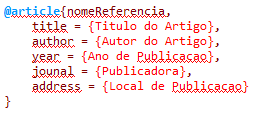
\includegraphics[scale=1]{./Imagens/capitulo_2/code_1.png}
	\end{center}
\end{figure}

tem-se como resultado:

\begin{equation}\label{equacao1}
	3x^2 = 2
\end{equation}

Está forma é muito útil quando você quer referenciar alguma equação ao longo do texto, pois com o comando \lstinline[language=TeX]|\label{}| você pode em qualquer local utilizar o \lstinline[language=TeX]|\ref{}| para referenciar aquele ``label'', por exemplo: ``Seja a equação \ref{equacao1} tem-se que...'' é possível fazer isso para todas as equações dentro do ambiente ``equation'', figuras, tabelas, basta alterar o que está escrito dentro do ``label'', e usar o ``ref'' para referenciar ela.

Outra forma de inserir equações matemáticas é utilizando \lstinline[language=TeX]|\[ \]| o que colocar dentro destes colchetes será centralizado, mas não sera enumerado, por exemplo:

\begin{figure}[htb]
	\begin{center}
		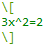
\includegraphics[scale=1.5]{./Imagens/capitulo_2/code_2.png}
	\end{center}
\end{figure}

terá como resultado:
\[
3x^2=2
\]
\subsection{Simbologia Matemática}
O LaTeX possui suporte a diversos símbolos matemáticos, desde simbologia como $\pm \div \bullet \bigtriangleup \neq \gg$ como também letras gregas como $\beta \gamma \delta \epsilon \varepsilon$ entre muitos outros. Para ver todos os símbolos matemáticos vá em ``View'' em ``Show'' e selecione ``Side Panel'', com isso irá abrir uma tela no canto lateral, navegue por ela e veja todos os símbolos que se pode adicionar, sempre fique atento em colocar os símbolos dentro de um ambiente matemático, se não será impossível compilar o projeto.
\subsection{Trabalhando com Equações}
O LaTeX tem suporte a diversas funções matemáticas, e alguns comandos que possibilitam o melhoramento dessas equações, a tabela

\begin{table}[htb]
	\IBGEtab{%
		\caption{Algumas Funções Matemáticas}%
		\label{tab_Cap2_equacoes}
	}{%
	\begin{tabular}{ccc|ccc}
		\toprule
		     Equação      &                   Código                    &      Resultado       &       Equação       &                Código                &     Resultado     \\ \midrule\midrule
		  Raiz Quadrada   &                \ba sqrt\{x\}                &      $\sqrt{x}$      & Integral Indefinida &             \ba int\{x\}             &     $\int{x}$     \\
		Raiz a Potencia N &              \ba sqrt[3]\{x\}               &    $\sqrt[3]{x}$     &  Integral Definida  & \ba int\_{2}\textasciicircum{3}\{x\} & $\int_{2}^{3}{x}$ \\
		    Somatoria     & \ba sum\_\{i=1\}\textasciicircum\{10\}\{x\} & $\sum_{i=1}^{10}{x}$ &       Fração        &          \ba frac\{x\}\{y\}          &   $\frac{x}{y}$   \\ \bottomrule
	\end{tabular}%
}{%
\fonte{Autoria Própria}%
}
\end{table}

Muitas outras funções podem ser obtidas indo em ``Math'' e em ``Math Function''. Observe que quando se utiliza uma função complexa dentro de uma tabela, como por exemplo a somatória, ela fica com a aparência um pouco ruim, com pouca organização, para resolver este problema, basta colocar antes da equação o comando \lstinline[language=TeX]|\displaystyle| assim ela ficará da seguinte forma:
\[
\sum_{i=1}^{10}{x}
\]

O mesmo vale para integrais, frações, raízes, entre outras.

\subsection{Teoremas, Definições e Provas}
Para realizar um teorema, uma definição ou uma prova, é utilizado o pacote amsthm, que adiciona ambientes próprios para cada um dessas funções, permitindo assim que fique mais visualmente agradável o trabalho, pois não existe uma norma especifica para este tipo de etapa. Estes ambientes são:
\begin{itemize}
	\item [plain] Teoremas, Lemas, Proposições, etc.
	\item [definition] Definições e Exemplos.
	\item [proof] Provas.
\end{itemize}

Para um exemplo de teorema, podemos colocar o teorema de Pitágoras que diz:
\begin{plain}
	Seja um triângulo retângulo qualquer, o quadrado do valor da hipotenusa é igual a soma dos quadrados dos catetos.
\end{plain}

Já para exemplo do ambiente definition, podemos usar:
\begin{definition}
	A função como a relação entre dois ou mais conjuntos, estabelecida por uma lei de formação, isto é, uma regra geral.
\end{definition}

Para um exemplo do ambiente proof, que serve pra provas, podemos usar:

\begin{proof}[Derivada de uma Função]
	Seja uma função $f(x)$ em um intervalo aberto $[a,b]$, então a função $f(x)$ possui uma derivada em $[a,b]$, podemos provar isso utilizando a definição de limites:
	\[
		f'(x) = \lim_{h\rightarrow 0} \frac{f(x + h) - f(x)}{h}
	\]
\end{proof}
\subsection{Tabulações}
\subsubsection{Matrizes}
Para a criação de matrizes existem os ambientes ``pmatrix'', ``bmatrix'', ``vmatrix'', ``Vmatrix'', ``matrix'' e ``array''. O ``pmatrix'' serve para a criação de matrizes com parenteses nas bordas, como por exemplo:
\[
\begin{pmatrix}
	2x & 3x \\ 
	x & 4x
\end{pmatrix} 
\]

o ``bmatrix'' serve para criar matrizes na forma de caixa, por exemplo:
\[
\begin{bmatrix}
2x & 3x \\ 
x & 4x
\end{bmatrix} 
\]

o ``vmatrix'' e o ``Vmatrix'' servem para criar matrizes com barras nas bordas, o primeiro com 1 barra, e o segundo com 2 barras, por exemplo: \\
\begin{center}
$
\begin{vmatrix}
2x & 3x \\ 
x & 4x
\end{vmatrix} 
$
\hspace*{2cm}
$
\begin{Vmatrix}
2x & 3x \\ 
x & 4x
\end{Vmatrix} 
$
\end{center}

o ``matrix'' cria uma matriz sem nenhuma borda
\[
\begin{matrix}
2x & 3x \\ 
x & 4x
\end{matrix}
\]

já o ``array'' é possível editar para colocar barras entre cada coluna ou linha, por exemplo:
\[
\begin{array}{c|ccc}
2x & 3y &2z & 4w\\ 
x & 4y & 3z & 8w \\ \hline
3x & 7y & 5z & 12w
\end{array}
\]
é possível também colocar o array dentro de um ``bmatrix'', ou ``pmatrix'' ou qualquer outra matriz, mas caso você deseje utilizar por exemplo, um lado de parentese e outro de colchete, é preciso usar as funções \lstinline|\left| e \lstinline|\right| acompanhado do simbolo que deseje, por exemplo, o código a seguir, apresenta o seguinte resultado:

\begin{figure}[htb]
	\begin{center}
		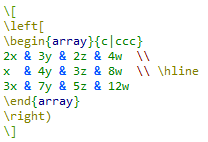
\includegraphics[scale=1]{./Imagens/capitulo_2/code_3.png}
	\end{center}
\end{figure}

\[
\left[
\begin{array}{c|ccc}
2x & 3y & 2z & 4w  \\
x  & 4y & 3z & 8w  \\ \hline
3x & 7y & 5z & 12w
\end{array}
\right)
\]

\subsubsection{Tabelas}
Para a utilização de Tabelas nas normas da ABNT é preciso usar os comandos:

\begin{figure}[htb]
	\begin{center}
		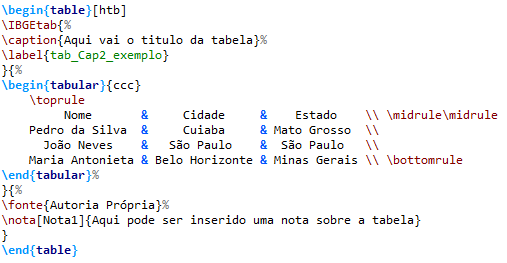
\includegraphics[scale=1]{./Imagens/capitulo_2/code_4.png}
	\end{center}
\end{figure}

Isto fornece a seguinte tabela:

\begin{table}[htb]
\IBGEtab{%
\caption{Aqui vai o titulo da tabela}%
\label{tab_Cap2_exemplo}
}{%
\begin{tabular}{ccc}
	\toprule
	     Nome       &     Cidade     &    Estado    \\ \midrule\midrule
	Pedro da Silva  &     Cuiaba     & Mato Grosso  \\
	  João Neves    &   São Paulo    &  São Paulo   \\
	Maria Antonieta & Belo Horizonte & Minas Gerais \\ \bottomrule
\end{tabular}%
}{%
\fonte{Autoria Própria}%
\nota[Nota1]{Aqui pode ser inserido uma nota sobre a tabela}
}
\end{table}



\subsection{Apresentação de Códigos de Programação}
Para a apresentação de códigos de programação, utiliza-se do pacote listings, ele é responsável por apresentar código em diferentes linguagens, com as fontes e detalhes específicos de cada linguagem, com destaques em suas palavras-chave ou em seus comentários. Para mudar as cores e outros detalhes da linguagem, olhe a parte ``Configurações de Linguagens de Programacao'' do preâmbulo.

Para utilizar este pacote, adicione-o inicialmente no preâmbulo e já será possível usa-lo através do ambiente lstlisting. Por exemplo:
\begin{lstlisting}[language = Java]
public main Codigo(){
 public void main[String args]{
  int calcular = 0;
  for(int i = 0; i <= 10; i++){
   calcular += i;
   System.out.printf("Ola Mundo! O valor: ", calcular);
  }
 }
}
\end{lstlisting}

Está normatização pode ser feita para quase todas as linguagens, algumas eu não tive sucesso em conseguir configurar, um exemplo é a própria linguagem TeX, que não tive sucesso na configuração. 
\section{Inserção de Imagens}
Para adicionar imagens, conforme as normas da ABNT, é necessário utilizar o código:

\begin{figure}[htb]
	\begin{center}
		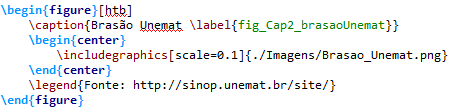
\includegraphics[scale=1]{./Imagens/capitulo_2/code_5.png}
	\end{center}
\end{figure}

Com este código, a imagem fica na seguinte forma:

\begin{figure}[htb]			
	\caption{Brasão Unemat \label{fig_Cap2_brasaoUnemat}}
	\begin{center}
		
\includegraphics[scale=0.1]{./Imagens/Brasao_Unemat.png}
	\end{center}
	\legend{Fonte: http://sinop.unemat.br/site/}
\end{figure}

 \begin{observacao}
 	Quanto as imagens é a sua organização, caso ela venha a ficar no fim de uma página, e não possui espaço para encaixa-la nesta pagina, ela automaticamente será enviada para  próxima página e ocupará o centro desta (caso não possua texto subsequente como um fim de capítulo).
\end{observacao}